
\documentclass{beamer}

\usetheme{Darmstadt}
\usecolortheme{beaver}
\setbeamertemplate{footline}[frame number]

\usepackage{ulem}
\usepackage{tikz}
\usepackage{subcaption}
\usepackage{booktabs}
\usepackage{subcaption}

%Information to be included in the title page:
\title{Combining Memory-Efficient Parallel SAT Solving and Distributed Clause Sharing}
\subtitle{Master Thesis}
\author{Ruben Götz}
%\institute{Overleaf}
\date{11.9.2025}

% 20-25 Minuten ist die Norm für einen Mastervortrag. 
% Eine kurze Einleitung für Menschen, die SAT Solving 
% schonmal gehört haben, ganz kurz der relevante 
% Stand der Technik, deine Contributions als Hauptteil 
% und die wichtigsten Ergebnisse aus der Evaluation 
% (dem kannst du denke ich viel Gewicht geben, weil 
% das dann auch den Schwerpunkt deiner MA spiegelt). 


\begin{document}

\frame{\titlepage}

\section{Introduction}
\begin{frame}{Introduction}
    \begin{block}{SAT Solving}
        Given a boolean formula (usually in CNF):
        \begin{itemize}
            \item Decide whether Formula is SAT
            \item Give assignment if Formula is SAT
        \end{itemize}
    \end{block}

    \begin{exampleblock}{$F = (a \lor b) \land (\lnot a \lor c \lor d)$}
        Is SAT for examplary assignment $a = false, b = true, c = false, d = false$
    \end{exampleblock}
\end{frame}

\begin{frame}{Introduction}
    \begin{block}{Usecases}
        \begin{itemize}
            \item Hardware and Software verification
            \item Automated Planning
            \item Scheduling
            \item Cryptoanalysis
            \item (explainable) AI
            \item Theorem Proving
            \item $\cdots$
        \end{itemize}
    \end{block}
\end{frame}

\section{State of the Art}
\begin{frame}{State of the Art}
    \begin{block}{Serial SAT solvers}
        \begin{itemize}
            \item Mostly based on CDCL algorithm
            \item i.e. learns conflict clauses
        \end{itemize}
    \end{block}

    \begin{block}{Parallel SAT solvers}
        \begin{itemize}
            \item Search Space Partitioning: Divide problem into disjoint subspaces
            \item Portfolio Solvers: Run multiple diverse serial solvers in parallel
            \item Increase efficiency by sharing clauses
            \item Distributed SAT solving is on the rise
            \item Annual SAT competition includes cloud track since 2020
            \item MallobSat
        \end{itemize}
    \end{block}
\end{frame}

\begin{frame}{State of the Art}
    \begin{block}{Memory-Efficiency SAT solving}
        \begin{itemize}
            \item Most research focuses on runtime
            \item Running independent solver engines comes with inherent memory redundancy
            \item[$\Rightarrow$] Gimsatul utilizes shared clauses in Memory
        \end{itemize}
    \end{block}
\end{frame}

\begin{frame}{MallobSat}
    \center
    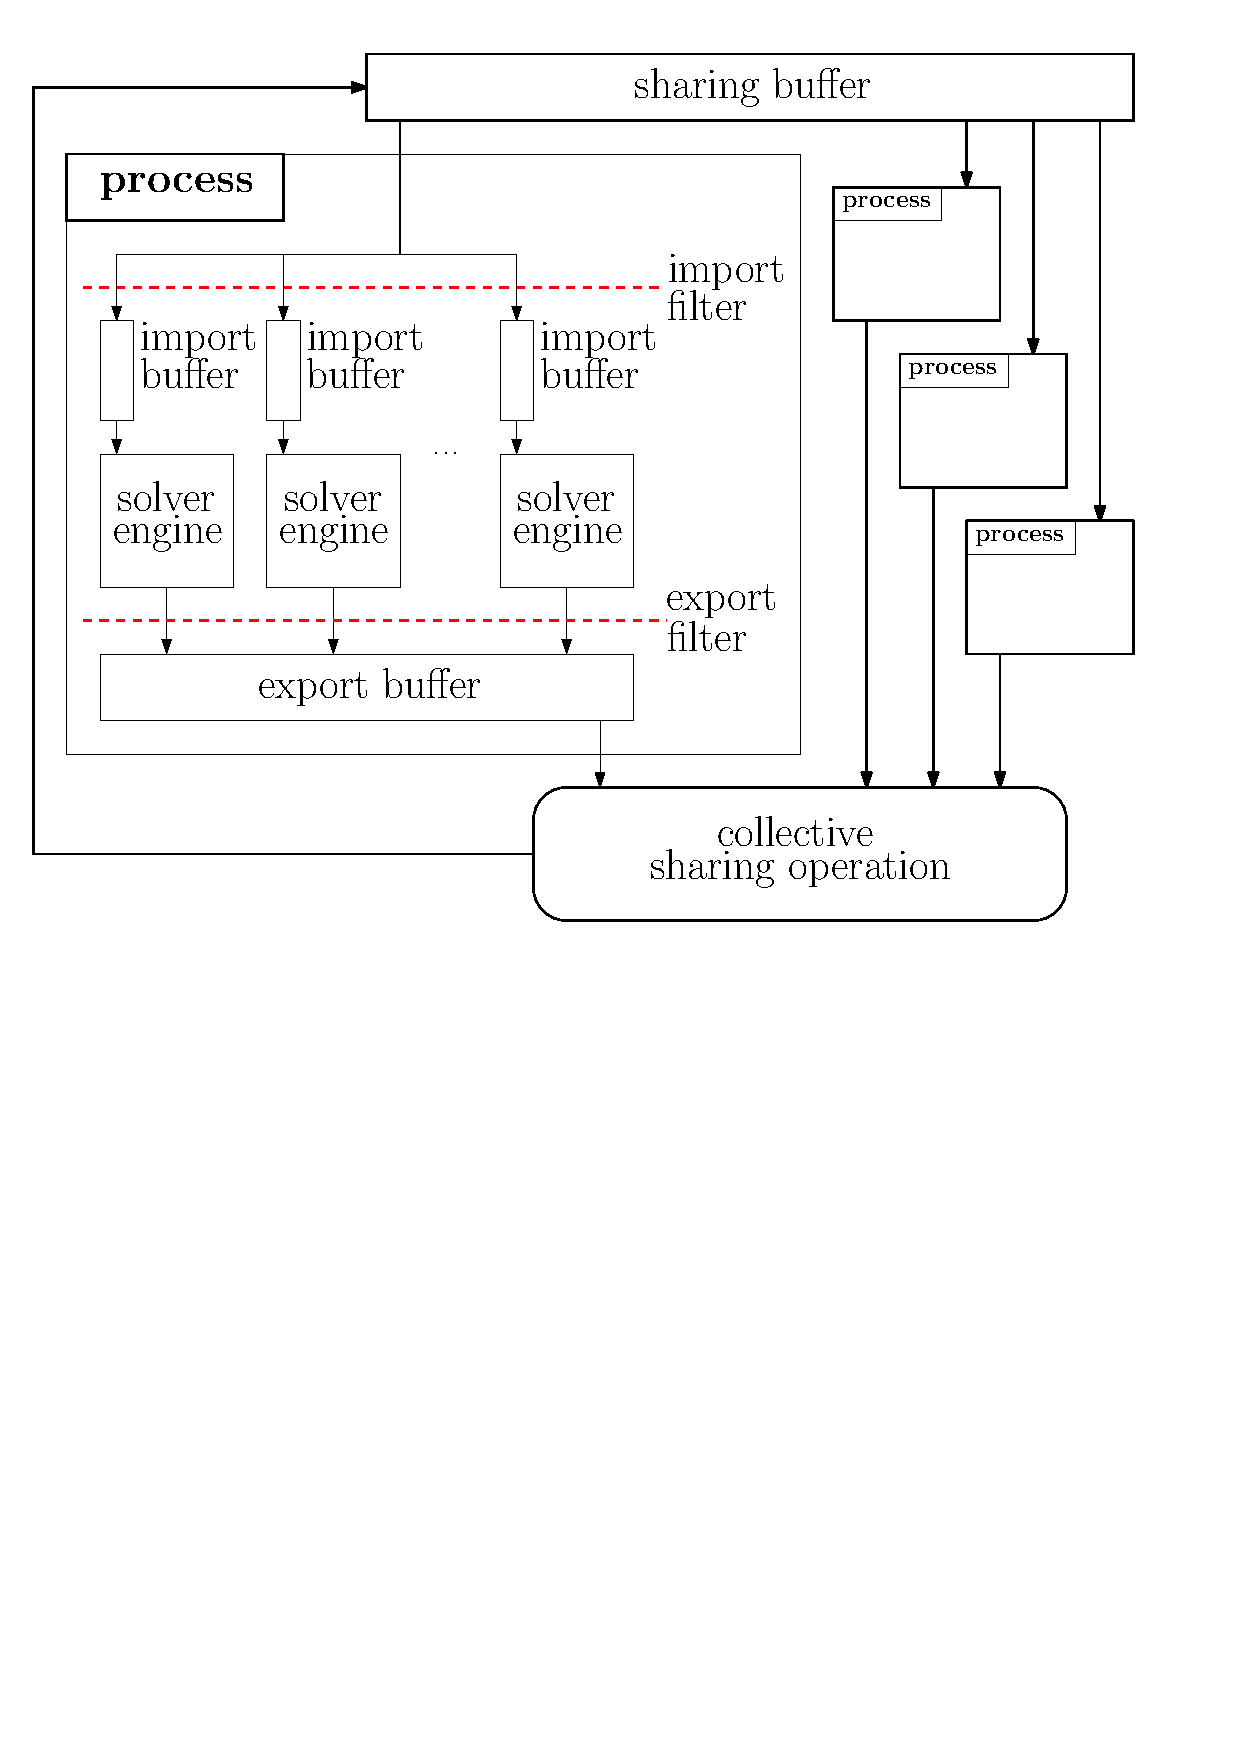
\includegraphics[scale=.45]{figures/mallob_architecture.pdf}
\end{frame}

\begin{frame}{Gimsatul}
    \center
    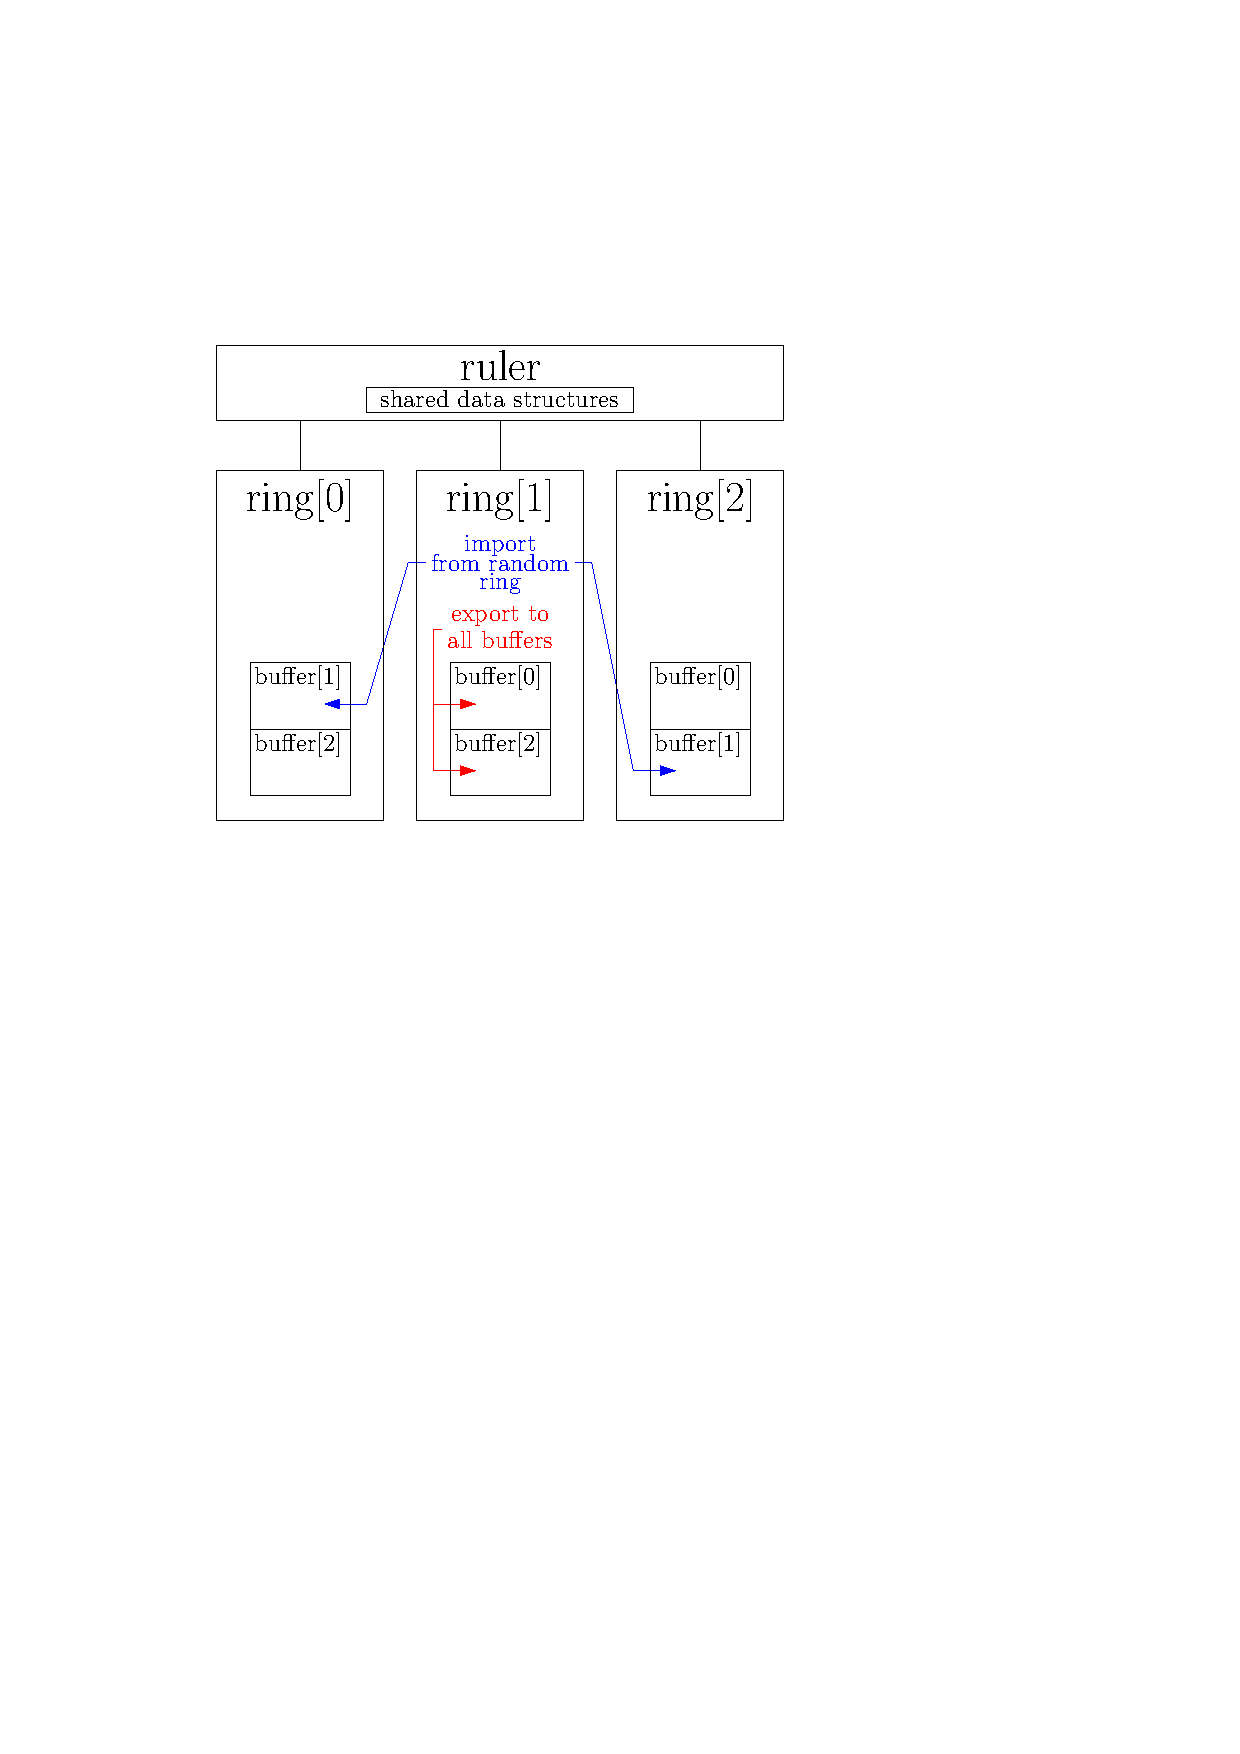
\includegraphics[scale=.8]{figures/gimsatul_architecture.pdf}
\end{frame}

\section{Contributions}
\begin{frame}{Contributions}
    \center
    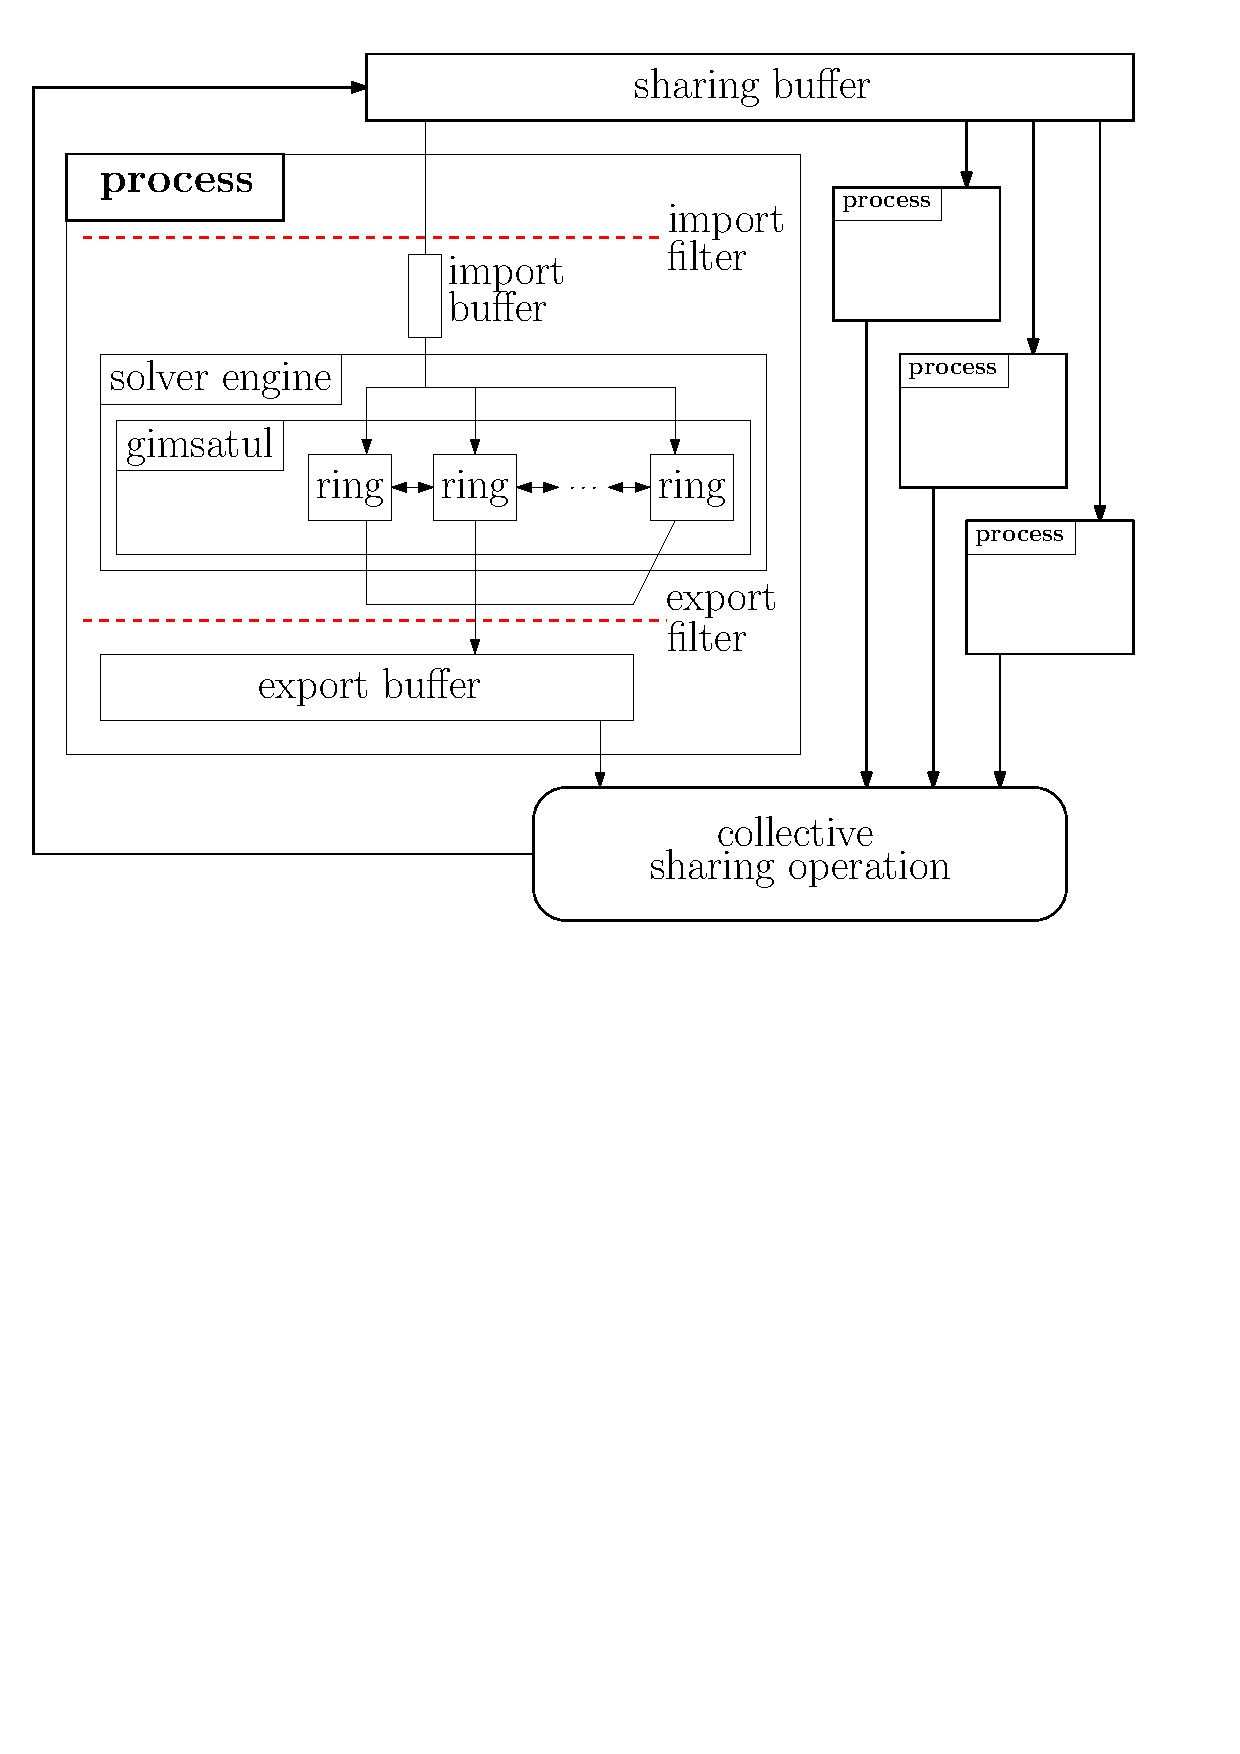
\includegraphics[scale=.45]{figures/architecture.pdf}
\end{frame}

\begin{frame}{Contributions}
    \begin{block}{Creating the Solver Engine}
        If Gimsatul is part of portfolio:
        \begin{itemize}
            \item Accumulate all $t'$ threads, that are defined to be Gimsatul
            \item Run Gimsatul with $t'$ threads
            \item MallobSat process runs with $t$ threads and $t - t' + 1$ solver engines
            \item extend Gimsatul's diversification
        \end{itemize}
    \end{block}
\end{frame}

\begin{frame}{Contributions}
    \begin{block}{Clause Export}
        \begin{itemize}
            \item All rings export externally if they export internally
            \item MallobSat's clause sharing mechanisms elegantly handles...
            \begin{itemize}
                \item[...] Clause filtering
                \item[...] Avoiding redundant clause sharing
            \end{itemize}
        \end{itemize}
    \end{block}

    \begin{block}{Clause Import}
        \begin{itemize}
            \item All rings import independently
            \item If there are conflicts, importing is skipped
            \item A ring imports at most as many clauses as there are rings in its Gimsatul instance
        \end{itemize}
    \end{block}
\end{frame}

\section{Experimental Evaluation}
\begin{frame}{Benchmarks \& Configuration}
    \begin{block}{Benchmarks}
        Benchmarks were provided by Iser and Jabs in 
        their Global Benchmark Database. Specifically, 
        we used the track \textit{main\_2024}.
    \end{block}

    \begin{block}{Configuration}
        \begin{itemize}
            \item Experiments done on SuperMUC
            \begin{itemize}
                \item 1 node contains 48 cores (96 Hardware threads)
                \item used up to 16 nodes (768 cores)
            \end{itemize}
            \item 1 Gimsatul instance per node
            \item 48 threads per node
            \item Search Only approach
            \begin{itemize}
                \item Deactivate pre- and inprocessing
                \item Run single dedicated preprocessing job in the beginning
                \item Replace jobs with preprocessed formula over time
            \end{itemize}
        \end{itemize}
    \end{block}
\end{frame}

\begin{frame}{Runtime}
    \center
    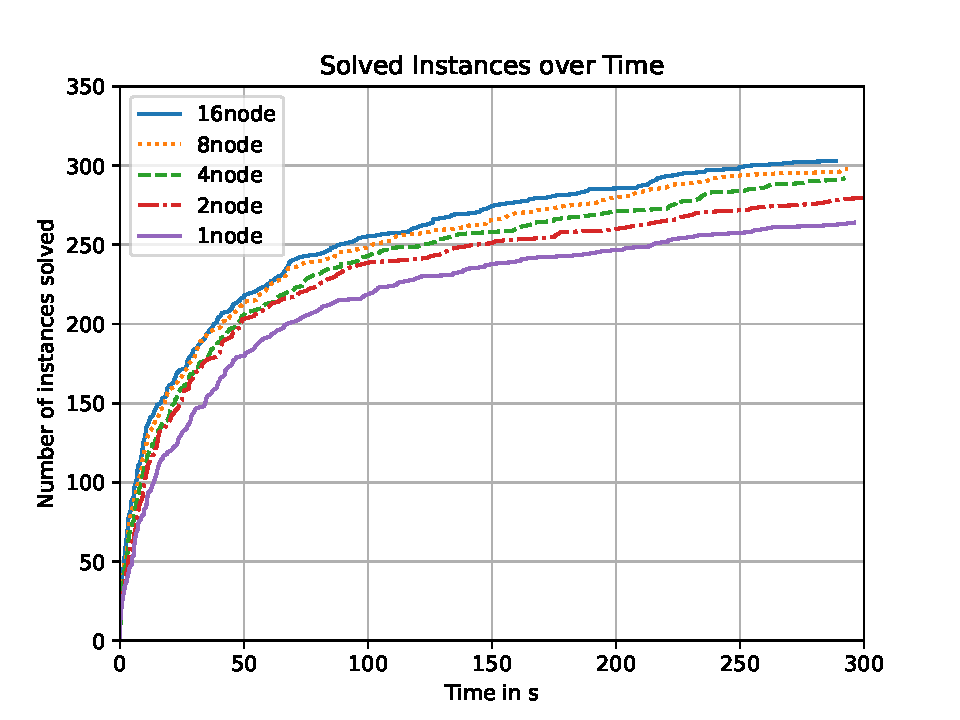
\includegraphics[scale=.55]{plots/cumulative_runtime/scalability_gim.pdf}
\end{frame}

\begin{frame}{Speedups}
    \center
    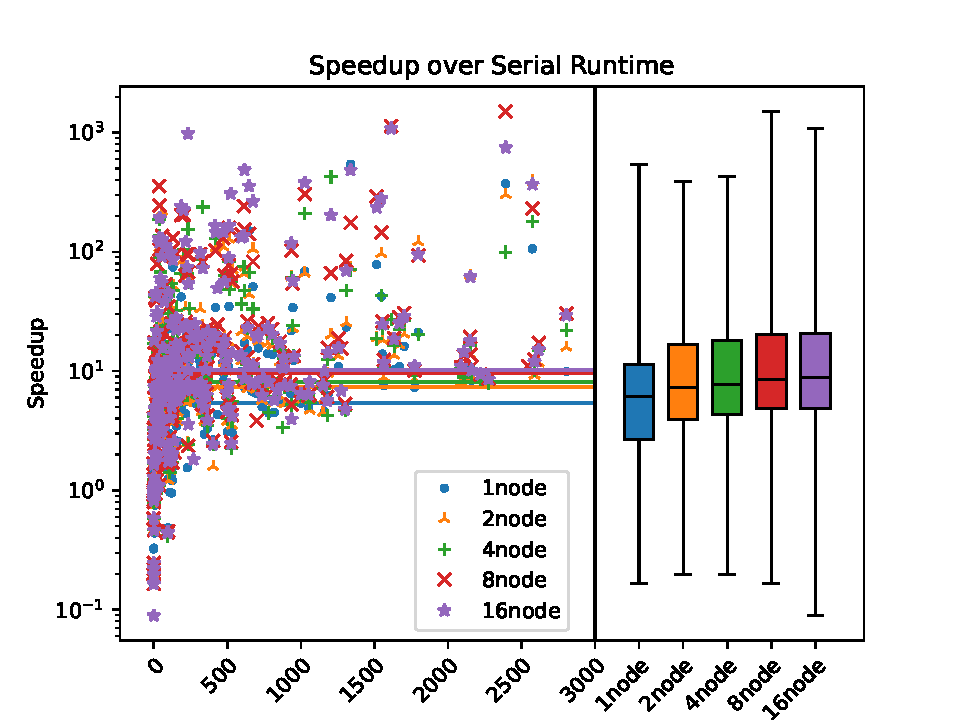
\includegraphics[scale=.3]{plots/speedups_gim.pdf}
    
    \begin{table}[!h]
        \center
        \begin{tabular}{ cccccc }
          \toprule
          \#cores & 1 & 2 & 4 & 8 & 16 \\
          gm Speedup & 5.357 & 7.384 & 8.146 & 9.720 & 10.260 \\
          \bottomrule
        \end{tabular}
        %\caption{Geometric mean speedups for number of cores.}
    \end{table}
\end{frame}

\begin{frame}{Comparison to MallobSat}
    \begin{figure}[!h]
      \center
      \begin{subfigure}[c]{.4\textwidth}
        \center
        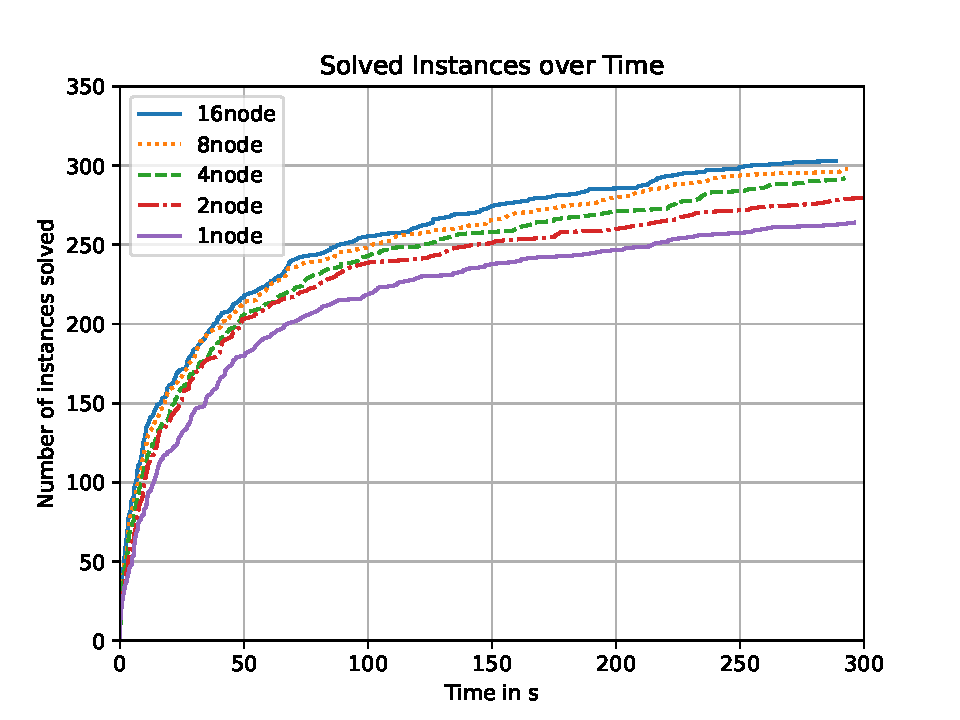
\includegraphics[scale=.3]{plots/cumulative_runtime/scalability_gim.pdf}
        \subcaption{Scalability of our approach}
      \end{subfigure}
      \hfill
      \begin{subfigure}[c]{.4\textwidth}
        \center
        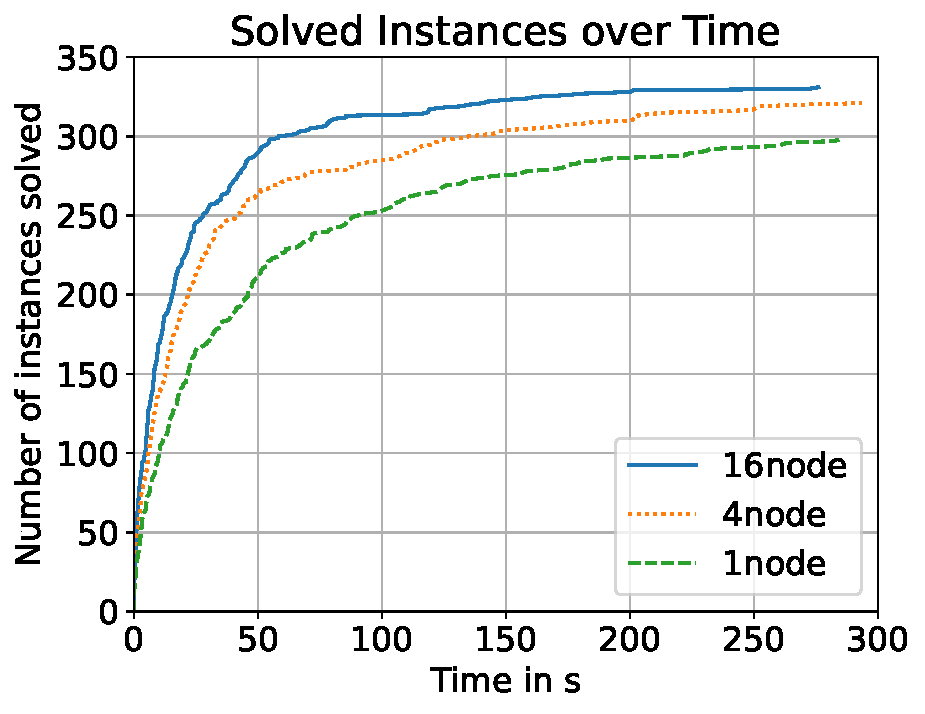
\includegraphics[scale=.3]{plots/cumulative_runtime/scalability_kis.pdf}
        \subcaption{Scalability of MallobSat}
      \end{subfigure}
      \caption{Scalability of our approach compared to MallobSat.}
    \end{figure}
\end{frame}

\begin{frame}{Comparison to MallobSat}
    \center
    \begin{figure}[c]{}
      \center
      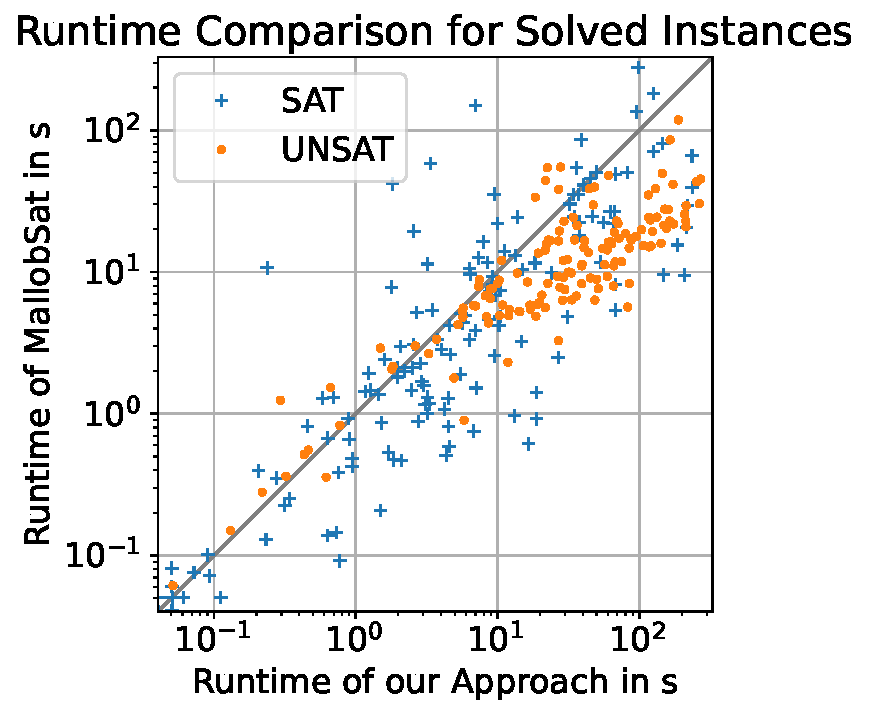
\includegraphics[scale=.45]{plots/square_runtime_compare/square_runtime_16node.pdf}
      \caption{Runtime Comparison between MallobSat and our approach, using 16 nodes.}
    \end{figure}
\end{frame}

\begin{frame}{}
    \center
    \begin{figure}[c]{Comparison to MallobSat}
        \center
        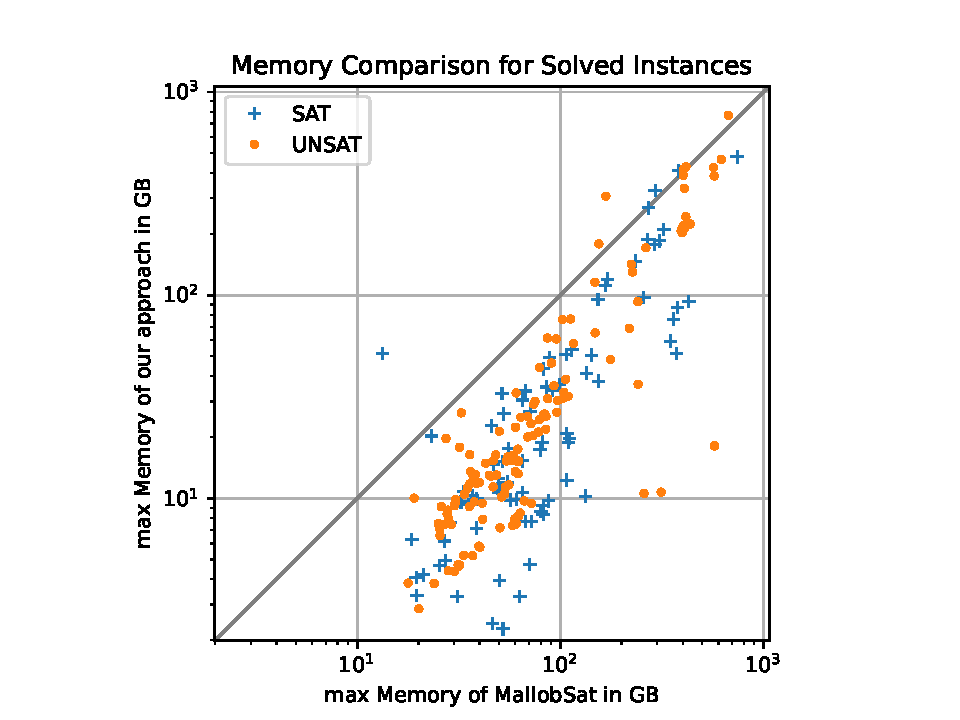
\includegraphics[scale=.45]{plots/square_mem_compare/square_mem_16node.pdf}
        \caption{Memory Comparison between MallobSat and our approach, using 16 nodes.}
    \end{figure}
\end{frame}

\begin{frame}{Comparison to MallobSat}
    \center
    \begin{figure}[c]{}
      \center
      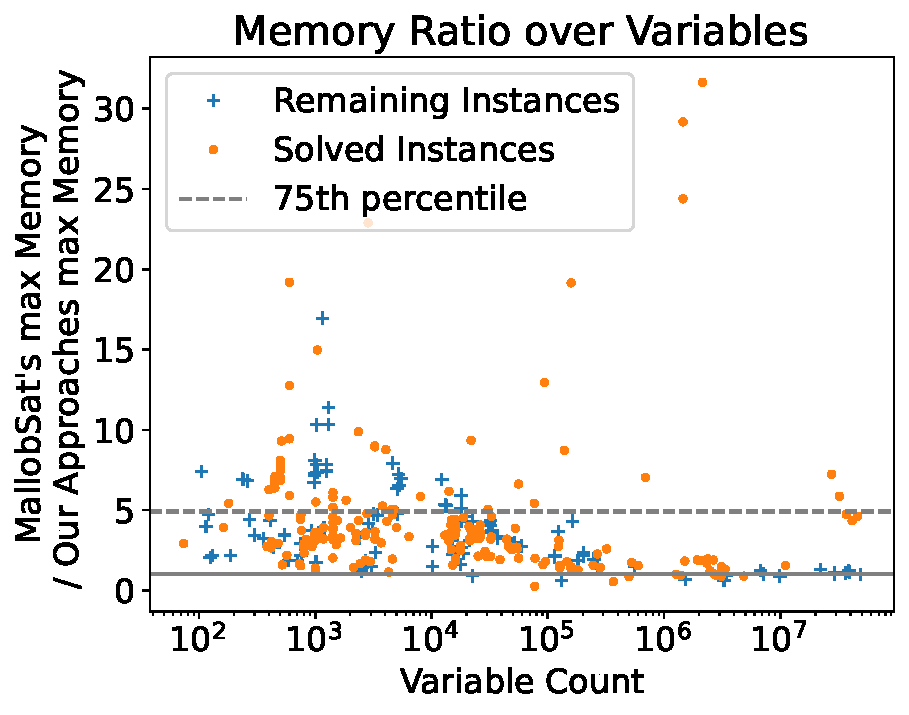
\includegraphics[scale=.45]{plots/16node_compare/mem_ratio_over_vars.pdf}
      \caption{Memory ratios between MallobSat and our approach, using 16 nodes. Each data point corresponds to a benchmark instance.}
    \end{figure}
\end{frame}

\begin{frame}{Comparison to MallobSat}
    \center
    \begin{figure}[c]{}
      \center
      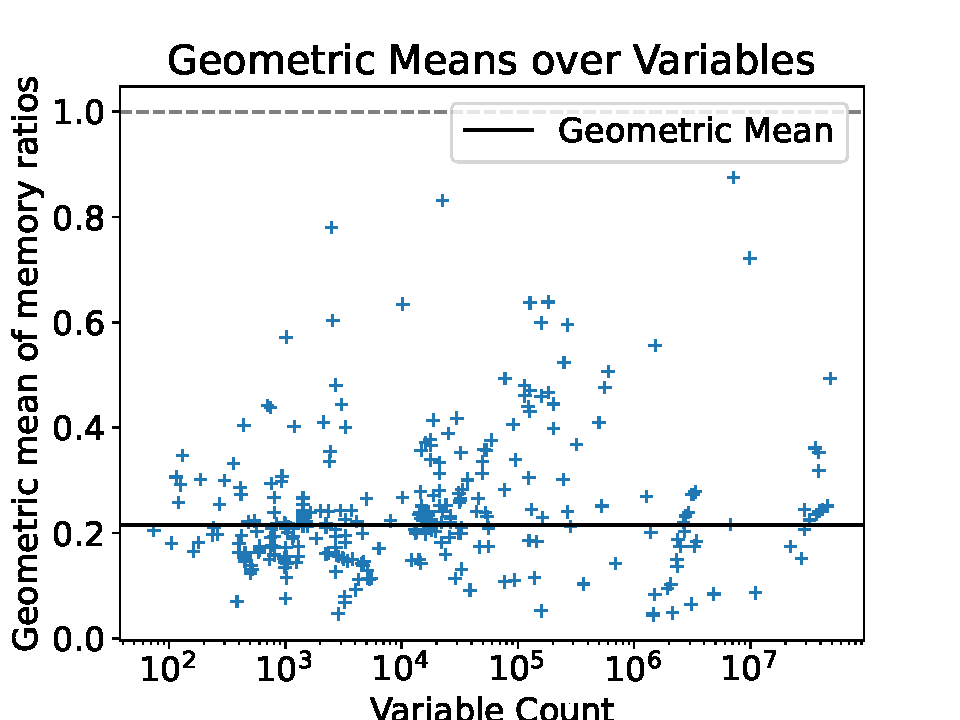
\includegraphics[scale=.425]{plots/16node_compare/mem_gm_over_vars.pdf}
      \caption{Geometric means for memory ratios between MallobSat and our approach per second, using 16 nodes. Each data point corresponds to a benchmark instance.}
    \end{figure}
\end{frame}

\begin{frame}{Comparison to MallobSat}
    \center
    \begin{figure}[c]{}
      \center
      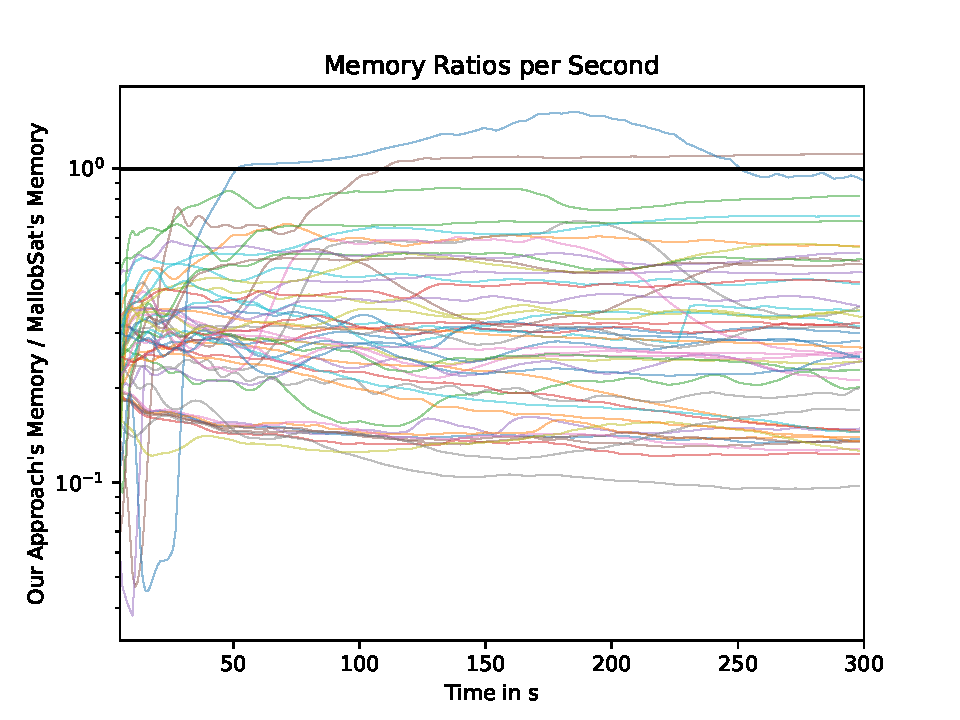
\includegraphics[scale=.45]{plots/16node_compare/mem_ratio_per_second.pdf}
      \caption{Memory ratios per second for all instances that reached the timeout of $300\,$s (both with MallobSat and our approach), using 16 nodes.} % The lines were smoothed, using a sliding window of size five seconds and calculating its geometric mean.
    \end{figure}
\end{frame}


\section{Conclusion}
\begin{frame}{Conclusion}
    \begin{block}{Summary}
        \begin{itemize}
            \item Integrated Gimsatul into MallobSat as solver engine
            \item Evaluated approach
        \end{itemize}
    \end{block}

    \begin{block}{Conclusion}
        \begin{itemize}
            \item Succeeded in stated goal to increase memory-efficiency
            \item Number for an Elevator Pitch: \textbf{0.25}
            \begin{itemize}
                \item gm of gm of Memory Ratios between MAllobSat and our approach
            \end{itemize}
            \item Runtime tradeoff
        \end{itemize}
    \end{block}
\end{frame}

\begin{frame}{Conclusion}
    \begin{table}[scale=.75]
        \center
        \begin{tabular}{ ccccc }
          \toprule
          \multicolumn{1}{c}{} & \multicolumn{2}{c}{Overall Used Memory} & \multicolumn{2}{c}{Normalized}\\
          \#cores & Our Approach & MallobSat & Our Approach & MallobSat \\
          \midrule
          48  & 0.149 & 0.089 & 7.140 & 4.256\\
          96  & 0.076 & -     & 7.306 & -\\
          192 & 0.039 & 0.026 & 7.583 & 5.036\\
          384 & 0.020 & -     & 7.780 & -\\
          768 & 0.010 & 0.006 & 7.766 & 4.924\\
          \bottomrule
        \end{tabular}
        \caption{Solved instances per GB of overall used memory in the middle and the same values normalized by the number of cores on the right.}
    \end{table}
\end{frame}


\end{document}
